\begin{figure*}
	\centering%
	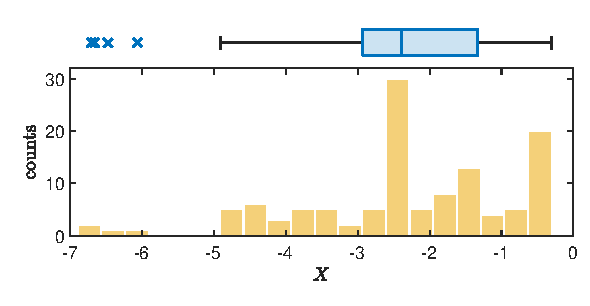
\includegraphics[width=\hsize]{\ROOTPATH/fig1.pdf}
	\caption{Radial acceleration relation (top) and mass discrepancy acceleration relation (bottom) for SPARC data and competing DM halo models. Each plot is divided in 50x50 equal bins. The baryonic centripetal acceleration $\SYMabar$ is inferred from luminosity observables while the total acceleration $\SYMatot$ is inferred independently from velocity fields. For DM halo models the total acceleration is composed of the predicted dark and inferred baryonic components, i.e. $\SYMatot = \SYMabar + \SYMaDM$. The corresponding solid curves are the best fits characterized by a specific $\mathfrak{a}_0$. \add{The histogram plots (upper row) show a Gaussian distribution of $\log_{10}(\SYMatot/\mathfrak{a}_0)$. The grayscale legend shows the number of points per bin (of a total 2396 for the 120 SPARC-galaxies used).}}%
	\label{fig:acceleration:grid}%
\end{figure*}
\begin{figure*}
	\figurenum{\arabic{figure}}
	\centering%
	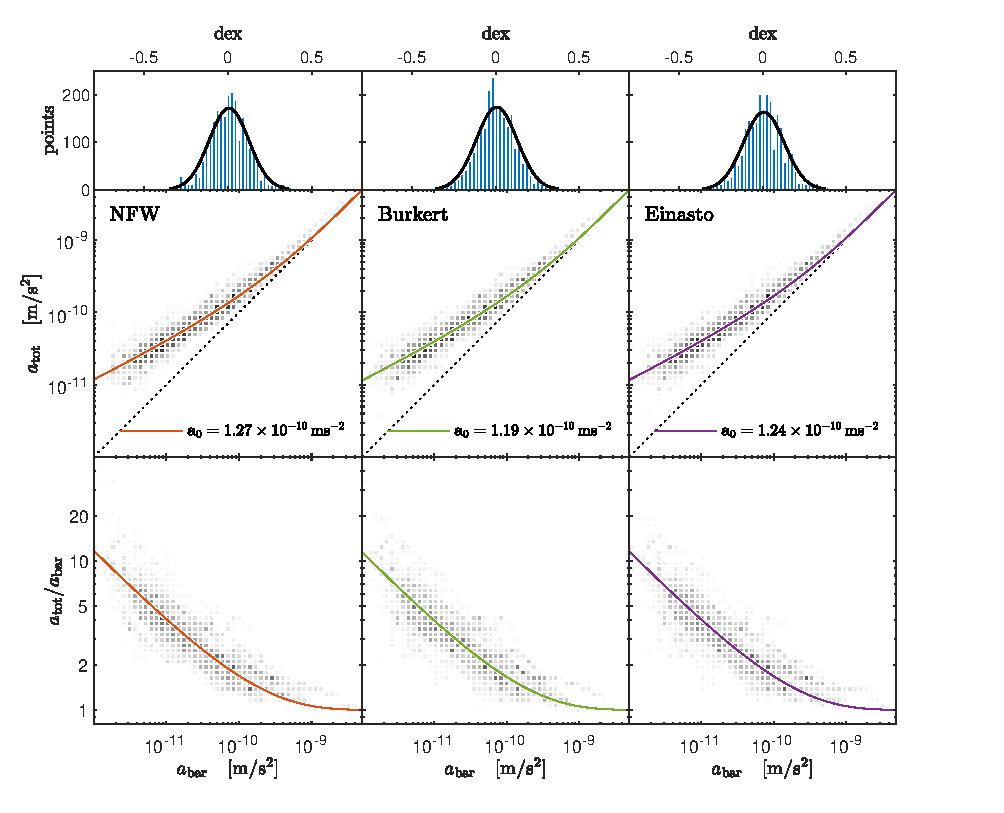
\includegraphics[width=\hsize]{\ROOTPATH/fig2.pdf}
	\caption{continue}
	\label{fig:acceleration:grid-b}%
\end{figure*}